%----------------------------------------------------------------------------------------
%	PACKAGES AND OTHER DOCUMENT CONFIGURATIONS
%----------------------------------------------------------------------------------------

\documentclass{article}

\usepackage{fancyhdr} % Required for custom headers
\usepackage{lastpage} % Required to determine the last page for the footer
\usepackage{extramarks} % Required for headers and footers
\usepackage[usenames,dvipsnames]{color} % Required for custom colors
\usepackage{graphicx} % Required to insert images
\usepackage{listings} % Required for insertion of code
\usepackage{courier} % Required for the courier font
\usepackage{lipsum} % Used for inserting dummy 'Lorem ipsum' text into the template
\usepackage{parskip}
% Margins
\topmargin=-0.45in
\evensidemargin=0in
\oddsidemargin=0in
\textwidth=6.5in
\textheight=9.0in
\headsep=0.25in

\linespread{1.1} % Line spacing

% Set up the header and footer
\pagestyle{fancy}
\chead{} % Top left header
\lhead{\hmwkClass\  \hmwkTitle} % Top center head
\rhead{} % Top right header
\lfoot{\lastxmark} % Bottom left footer
\cfoot{} % Bottom center footer
\rfoot{Page\ \thepage\ of\ \protect\pageref{LastPage}} % Bottom right footer
\renewcommand\headrulewidth{0.4pt} % Size of the header rule
\renewcommand\footrulewidth{0.4pt} % Size of the footer rule

\setlength\parindent{0pt} % Removes all indentation from paragraphs

%----------------------------------------------------------------------------------------
%	CODE INCLUSION CONFIGURATION
%----------------------------------------------------------------------------------------

% \definecolor{MyDarkGreen}{rgb}{0.0,0.4,0.0} % This is the color used for comments
\lstloadlanguages{C} % Load C syntax for listings, for a list of other languages supported see: ftp://ftp.tex.ac.uk/tex-archive/macros/latex/contrib/listings/listings.pdf
\lstset{language=C,frame=single,keywordstyle=[1]\color{Blue}\bf} % Use C in this example      



\newcommand{\csnippet}[2]{
\begin{itemize}
\item[]\lstinputlisting[caption=#2,label=#1]{#1.c}
\end{itemize}
}

%----------------------------------------------------------------------------------------
%	DOCUMENT STRUCTURE COMMANDS
%----------------------------------------------------------------------------------------

% Header and footer for when a page split occurs within a problem environment
\newcommand{\enterProblemHeader}[1]{
\nobreak\extramarks{#1}{#1 continued on next page\ldots}\nobreak
\nobreak\extramarks{#1 (continued)}{#1 continued on next page\ldots}\nobreak
}

% Header and footer for when a page split occurs between problem environments
\newcommand{\exitProblemHeader}[1]{
\nobreak\extramarks{#1 (continued)}{#1 continued on next page\ldots}\nobreak
\nobreak\extramarks{#1}{}\nobreak
}

\setcounter{secnumdepth}{0} % Removes default section numbers
\newcounter{homeworkProblemCounter} % Creates a counter to keep track of the number of problems

\newcommand{\homeworkProblemName}{}
\newenvironment{homeworkProblem}[1][Problem \arabic{homeworkProblemCounter}]{ % Makes a new environment called homeworkProblem which takes 1 argument (custom name) but the default is "Problem #"
\stepcounter{homeworkProblemCounter} % Increase counter for number of problems
\renewcommand{\homeworkProblemName}{#1} % Assign \homeworkProblemName the name of the problem
\section{\homeworkProblemName} % Make a section in the document with the custom problem count
\enterProblemHeader{\homeworkProblemName} % Header and footer within the environment
}{
\exitProblemHeader{\homeworkProblemName} % Header and footer after the environment
}

\newcommand{\problemAnswer}[1]{ % Defines the problem answer command with the content as the only argument
\noindent\framebox[\columnwidth][c]{\begin{minipage}{0.98\columnwidth}#1\end{minipage}} % Makes the box around the problem answer and puts the content inside
}

\newcommand{\homeworkSectionName}{}
\newenvironment{homeworkSection}[1]{ % New environment for sections within homework problems, takes 1 argument - the name of the section
\renewcommand{\homeworkSectionName}{#1} % Assign \homeworkSectionName to the name of the section from the environment argument
\subsection{\homeworkSectionName} % Make a subsection with the custom name of the subsection
\enterProblemHeader{\homeworkProblemName\ [\homeworkSectionName]} % Header and footer within the environment
}{
\enterProblemHeader{\homeworkProblemName} % Header and footer after the environment
}

%----------------------------------------------------------------------------------------
%	NAME AND CLASS SECTION
%----------------------------------------------------------------------------------------

\newcommand{\hmwkTitle}{Assignment\ \#2} % assignment title
\newcommand{\hmwkDueDate}{Monday,\ November\ 16,\ 2014} % due date
\newcommand{\hmwkClass}{Programming Concurrent Systems} % class
\newcommand{\hmwkClassTime}{} % lecture time
\newcommand{\hmwkClassInstructor}{} % lecturer
\newcommand{\hmwkAuthorName}{Alyssa - Ilias} %name

%----------------------------------------------------------------------------------------
%	TITLE PAGE
%----------------------------------------------------------------------------------------

\title{
\vspace{2in}
\textmd{\textbf{\hmwkClass:\ \hmwkTitle}}\\
\normalsize\vspace{0.1in}\small{Due\ on\ \hmwkDueDate}\\
\vspace{0.1in}\large{\textit{\hmwkClassInstructor\ \hmwkClassTime}}
\vspace{3in}
}

\author{\textbf{\hmwkAuthorName}}


%----------------------------------------------------------------------------------------

\begin{document}

\maketitle

%----------------------------------------------------------------------------------------
%	TABLE OF CONTENTS
%----------------------------------------------------------------------------------------

%\setcounter{tocdepth}{1} % Uncomment this line if you don't want subsections listed in the ToC

%\newpage
%\tableofcontents
\newpage

%----------------------------------------------------------------------------------------
%	Introduction
%----------------------------------------------------------------------------------------
\begin{homeworkProblem}[Introduction]
	For this assignment, we were asked to parallelize our previous heat dissipation implementation
	using OpenMP directives. Moreover using the same framework we had to implement and parallel version
	of the merge sort. Finally we were asked to implement a vector of vectors of different lengths and
	experiment with the scheduling of OpenMP.

\end{homeworkProblem}
%----------------------------------------------------------------------------------------
%	Heat
%----------------------------------------------------------------------------------------

% To have just one problem per page, simply put a \clearpage after each problem

\begin{homeworkProblem}[Heat dissipation | OpenMP]
\textbf{Solution description}

We also parallelize the reduction step as shown in the snippet below.

\csnippet{reduction}{Reduction using omp directive}

\textbf{Evaluation - Experiments}

We run our experiments on the DAS-4 system using a normal node which has 8 physical cores.

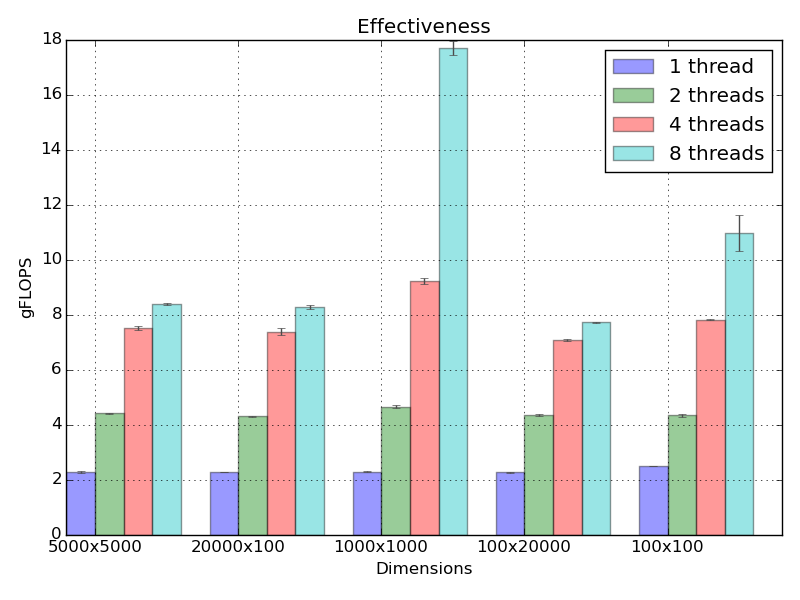
\includegraphics[width=0.75\columnwidth]{effectivness.png}


The figure above shows the effectivness of the parallelism. The experiments where made with the following parameters:

\begin{verbatim}
./heat -e 0.0 -i 2000 -k 2001
\end{verbatim}

Note that for the 5000x5000 we instead used -i 500 to normalize the graph a bit. Note that we achieve our biggest flops/s ratio
on the 1000x1000 experiment also having a superlinear performance with a value of 1.800922e+10. 

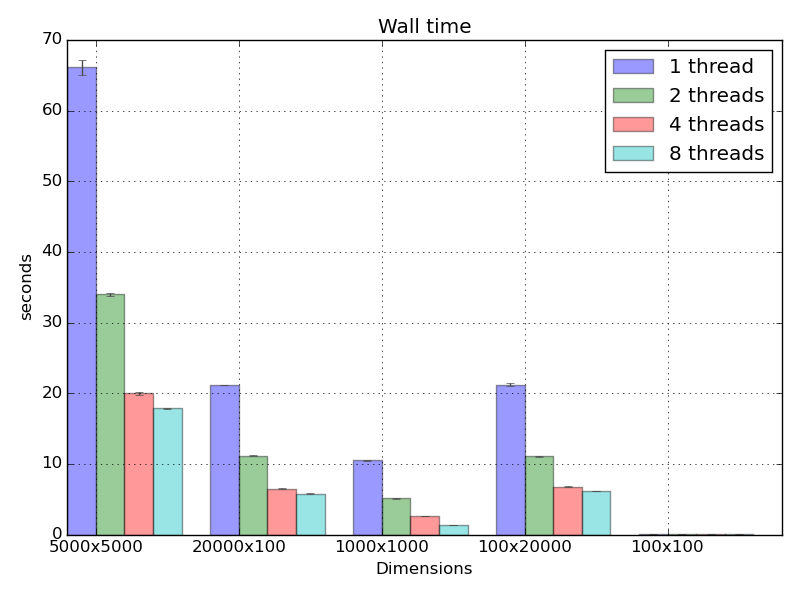
\includegraphics[width=0.75\columnwidth]{walltime.png}

This figure depicts the basic execution times for different numbers of cores and input sizes. Our fastest execution is ofcourse on the
100x100 image which is small enough for all of it to fit in a small cache. 

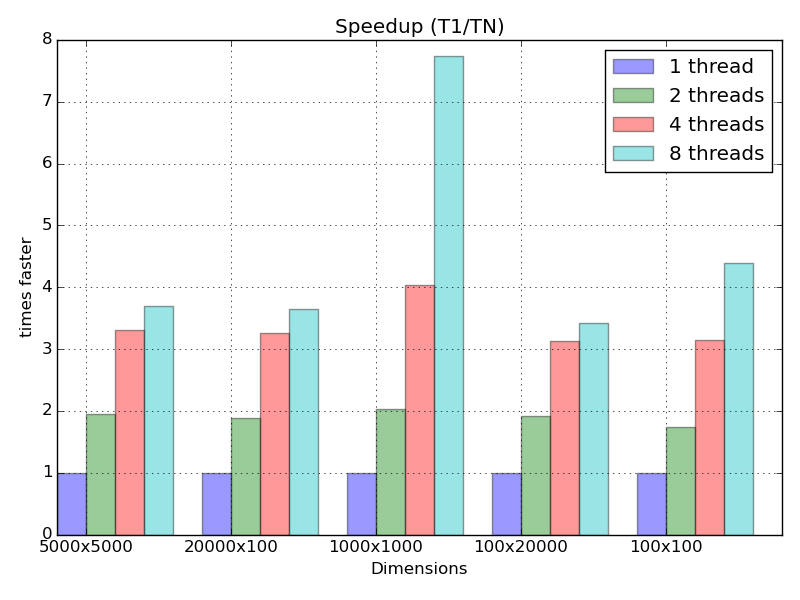
\includegraphics[width=0.75\columnwidth]{speedups.png} 

Here we show the speedups achieved by different core usage. Note that our basis execution is the multithreaded program for 1 thread. Interestingly enough the difference of the OpenMP implementation for 1 thread and our sequantial version is really small. So the speedups
would be effectivly the same. We show this on the following two figures.

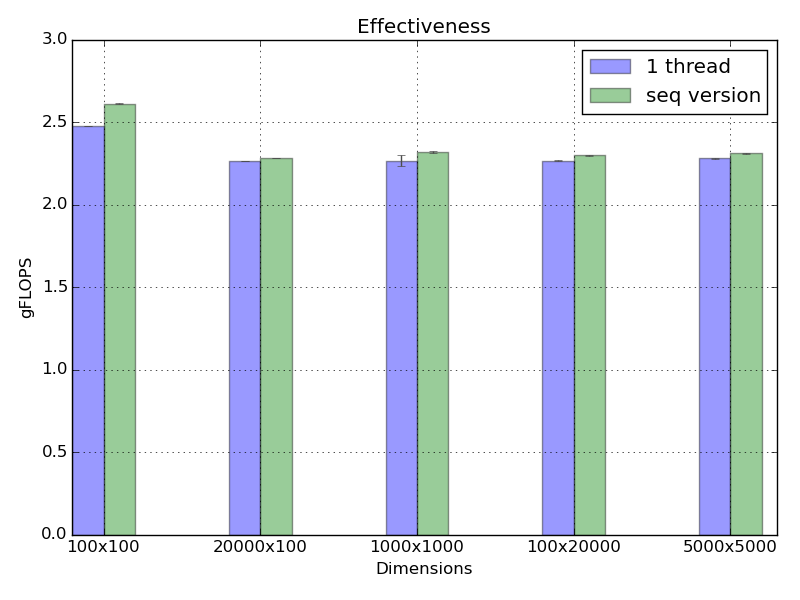
\includegraphics[width=0.75\columnwidth]{effcmp.png} 

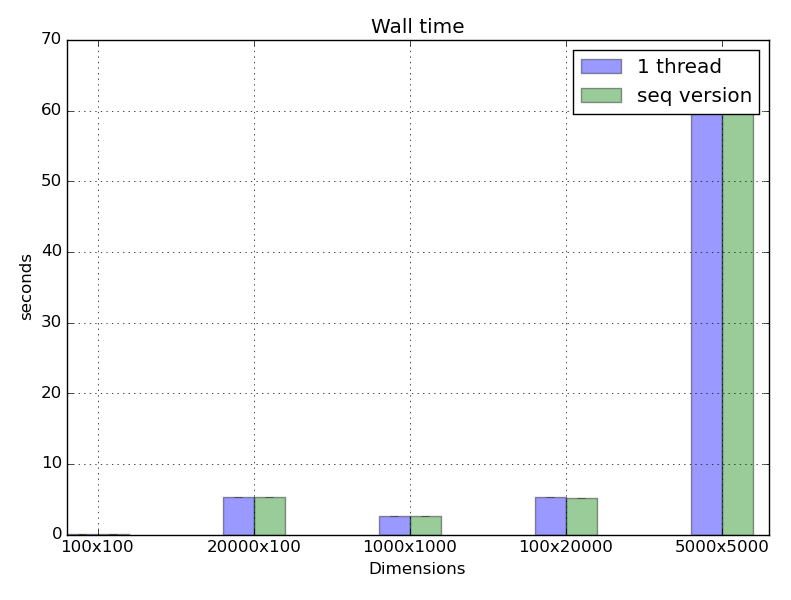
\includegraphics[width=0.75\columnwidth]{wallcmp.png}

Finally without neglecting the reduction computation we provide some graphs on the experiments we did. Since our implementation also uses concurrency to compute the reduction step as shown below, the reduction computation causes some overhead as expected but on the other hand very little, especially when using more than one threads. This means that we still achieve superlinear performance as the speedup figure below depicts. Note that for the experiments we used the worst case scenario which is doing the reduction step at every iteration (-k 1).

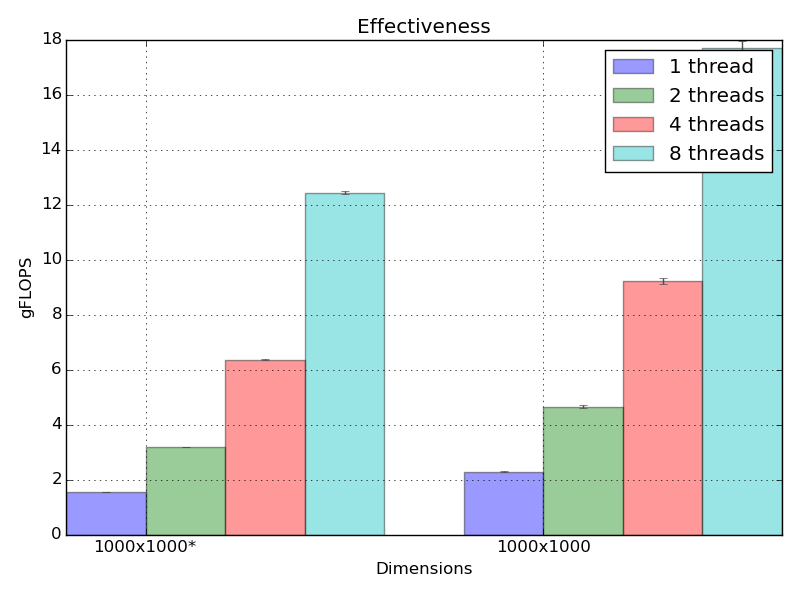
\includegraphics[width=0.75\columnwidth]{reducecmp.png} 

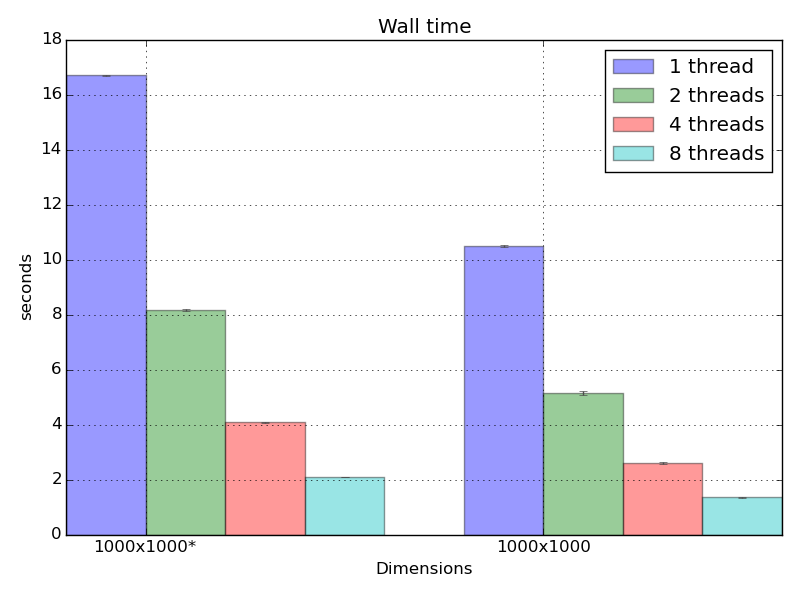
\includegraphics[width=0.75\columnwidth]{reducecmpwt.png}

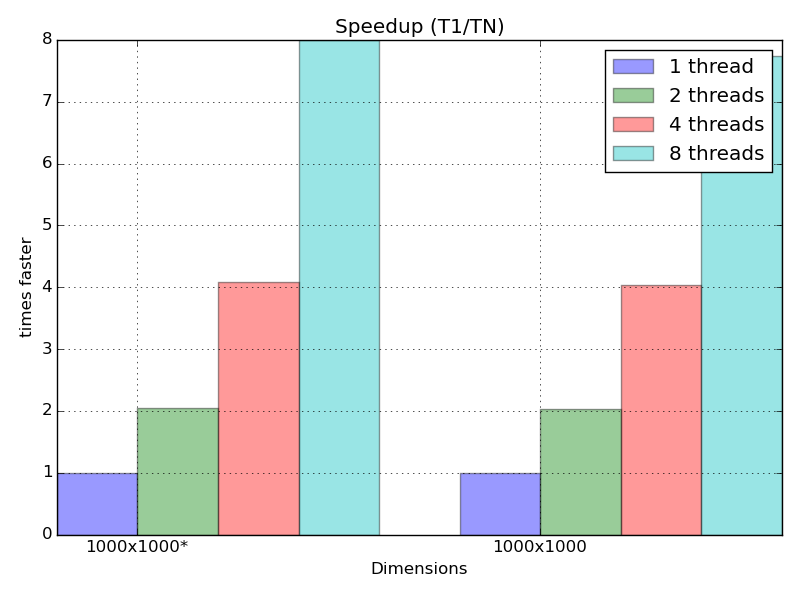
\includegraphics[width=0.75\columnwidth]{speedupwrd.png} 

Note that the 1000x1000* means these results include reduction computation. 

\end{homeworkProblem}

%----------------------------------------------------------------------------------------
%	Merge
%----------------------------------------------------------------------------------------

\begin{homeworkProblem}[Mergesort]
\textbf{Solution description}

solution desc here

\textbf{Evaluation}

experiments here

\end{homeworkProblem}

%----------------------------------------------------------------------------------------

\end{document}
